\documentclass[12pt,letterpaper]{article}
\usepackage[utf8]{inputenc}
\usepackage[spanish]{babel}
\usepackage{amsmath}
\usepackage{subcaption}
\usepackage{amsfonts}
\usepackage{amssymb}
\usepackage{listings}
\usepackage{graphicx}
\usepackage[left=2cm,right=2cm,top=2cm,bottom=2cm]{geometry}

\title{\textsc{Minería de Texto}}
\author{\textsc{Fabiola Vázquez}}

\setlength{\parindent}{0cm}

\begin{document}
\maketitle
\begin{abstract}
\begin{center}
El objetivo de esta tarea es analizar un libro te texto, mediante   las palabras, letras, personajes y  sentimientos que se mencionan. Se utilizan gráficas de barras y figuras, como los word clouds, para representar mejor, de una forma visual, estos resultados.
\end{center}
\end{abstract}
\hrule
\section{Introducción}
La minería de textos extrae información útil e interesante de textos, como lo pueden ser  de páginas web, documentos, artículos. En este caso, se realizó un estudio de la novela \textit{Alice's Adventures in Wonderland} \cite{alice} con el software estadístico R versión 4.0.2 \cite{R} en el IDE \textbf{R Studio} \cite{rstudio}. Se analizan las palabras, letras más frecuentes del libro, así como también, los sentimientos que se mencionan en él. 

\section{Análisis del texto}
La novela se extrajo de la librería electrónica Project Gutenberg, de la siguiente manera.
\begin{center}
\begin{lstlisting}[language=R]
library(gutenbergr)
alice <- gutenberg_download(c(11))
\end{lstlisting}
\end{center}
Una vez cargado, procedemos a crear dos listas que contengan los caracteres y las palabras de nuestro libro, respectivamente.
\begin{lstlisting}[language=R]
letras = alice %>% unnest_tokens(chars, text, "characters") 
palabras = alice%>% unnest_tokens(word, text, "words")
\end{lstlisting}

\subsection{Análisis de caracteres}
De nuestra lista de letras, no solo aparecen letras, si no también números, en el cuadro \ref{caracteres} aparecen los números cero y tres con frecuencia uno. Para el análisis, quitamos esos valores no deseados y procedemos a trabajar únicamente con las letras.
\begin{table}
\centering
\caption{Fragmento de la tabla de frecuencias de los caracteres que aparecen en el libro.}
\label{caracteres}
\begin{tabular}{ccc}
  \hline
 &Caracter & Frecuencia\\ 
  \hline
1& 0 &   1 \\ 
2&  3 &   1 \\ 
3& a & 8 791 \\ 
4& b & 1 475 \\ 
5& c & 2 399 \\ 
6& d & 4 931 \\ 
   \hline
\end{tabular}
\end{table}
\begin{table}
\centering
\caption{Fragmento de la tabla de frecuencias de las palabras que aparecen en el libro.}
\label{caracteres}
\begin{tabular}{ccc}
  \hline
 & Palabra & Frecuencia \\ 
  \hline
1 & the & 1 644 \\ 
  2 & and & 872 \\ 
  3 & to & 729 \\ 
  4 & a & 632 \\ 
  5 & she & 541 \\ 
  6 & it & 530 \\ 
  7 & of & 514 \\ 
  8 & said & 462 \\ 
   \hline
\end{tabular}
\end{table}

En la figura \ref{letras} podemos apreciar que la letra que tiene menor frecuencia es la letra \textbf{z} y la de mayor frecuencia es la \textbf{e}. El libro contiene 107 721 letras, de las cuales 13 576 son la letra \textbf{e}, eso quiere decir que son aproximadamente el 13\% de las letras.


\begin{figure}
\centering
\caption{Gráfica de barras de las frecuencias de caracteres.}
\label{letras}
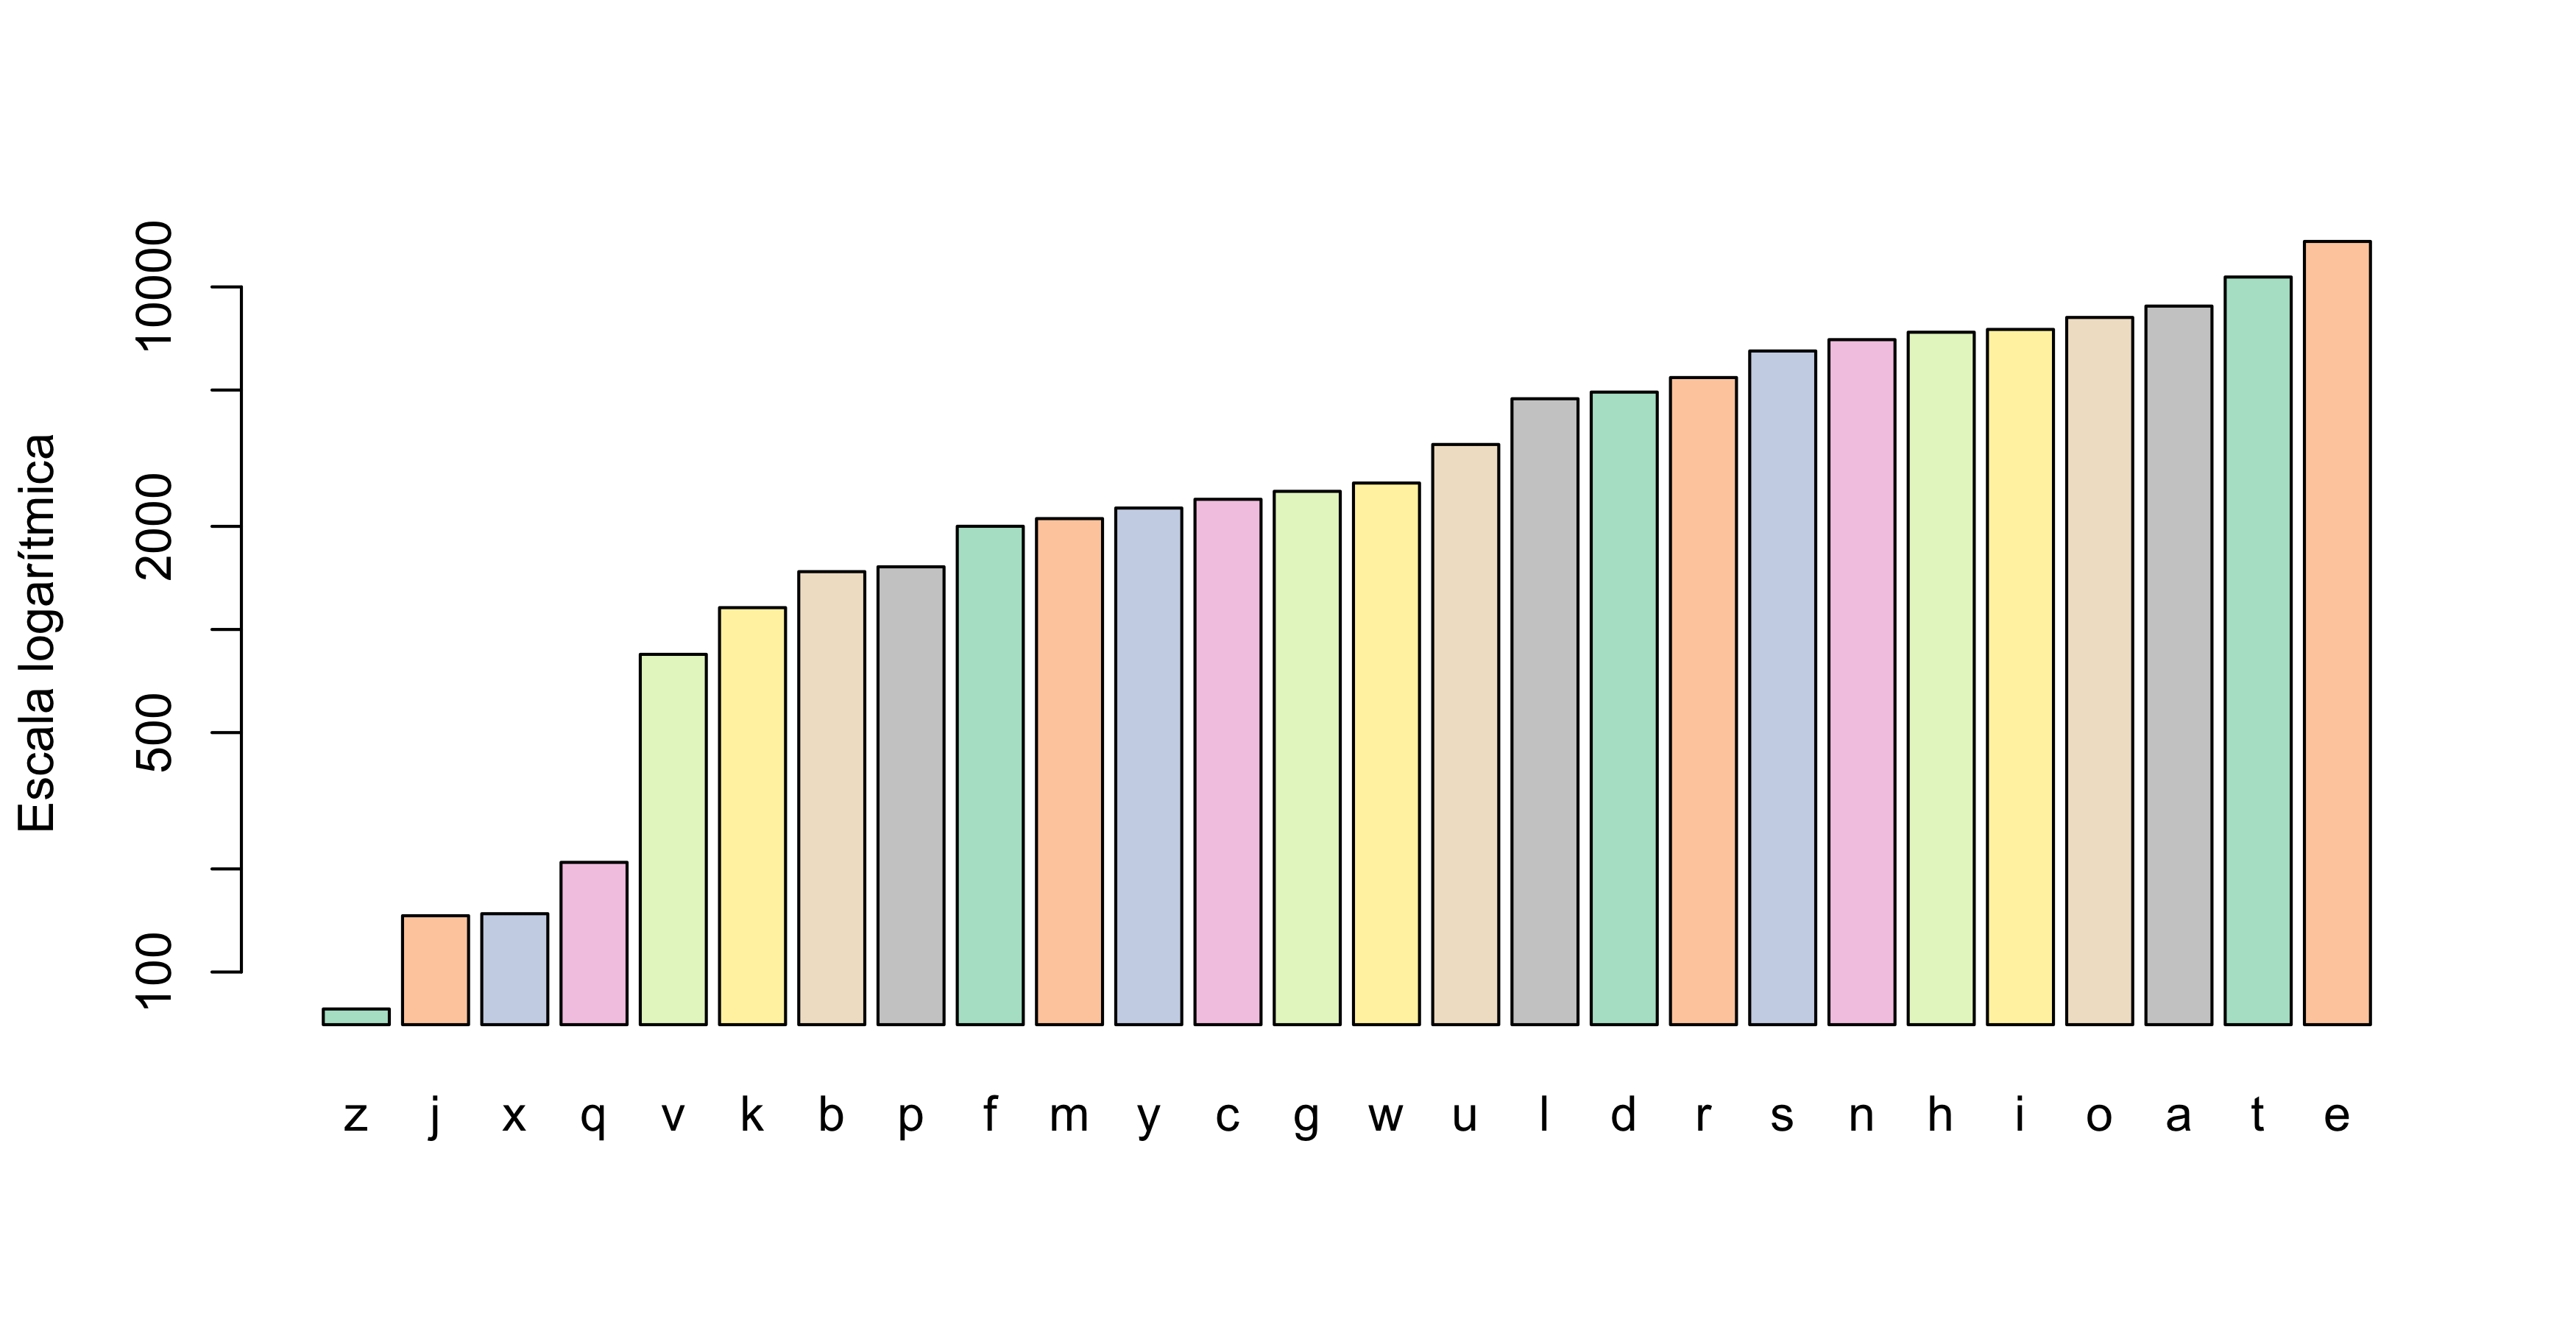
\includegraphics[scale=0.1]{Letras.png}
\end{figure}

\subsection{Análisis de palabras}
Se realizó una tabla de frecuencias de las palabras que aparecen en el libro y se obtuvo la figura \ref{Palabras}, en donde apreciamos que aparecen palabras del tipo artículo, pronombres, etcétera. Por ejemplo, la palabra \textit{the} tiene una frecuencia de 1 644. Para una mejor apreciación, quitamos dichas palabras, el gráfico correspondiente aparece en la figura  \ref{Palabrasmas}.
Otra manera de visualizar las palabras más frecuentes del libro, es usando un \textit{word cloud}, donde, las palabras de mayor tamaño son aquellas que tienen una frecuencia mayor en el texto,  como lo podemos apreciar en la figura \ref{cloudpalabras}.
\begin{figure}
\centering
\caption{Palabras más frecuentes en el libro.}
\label{Palabras}
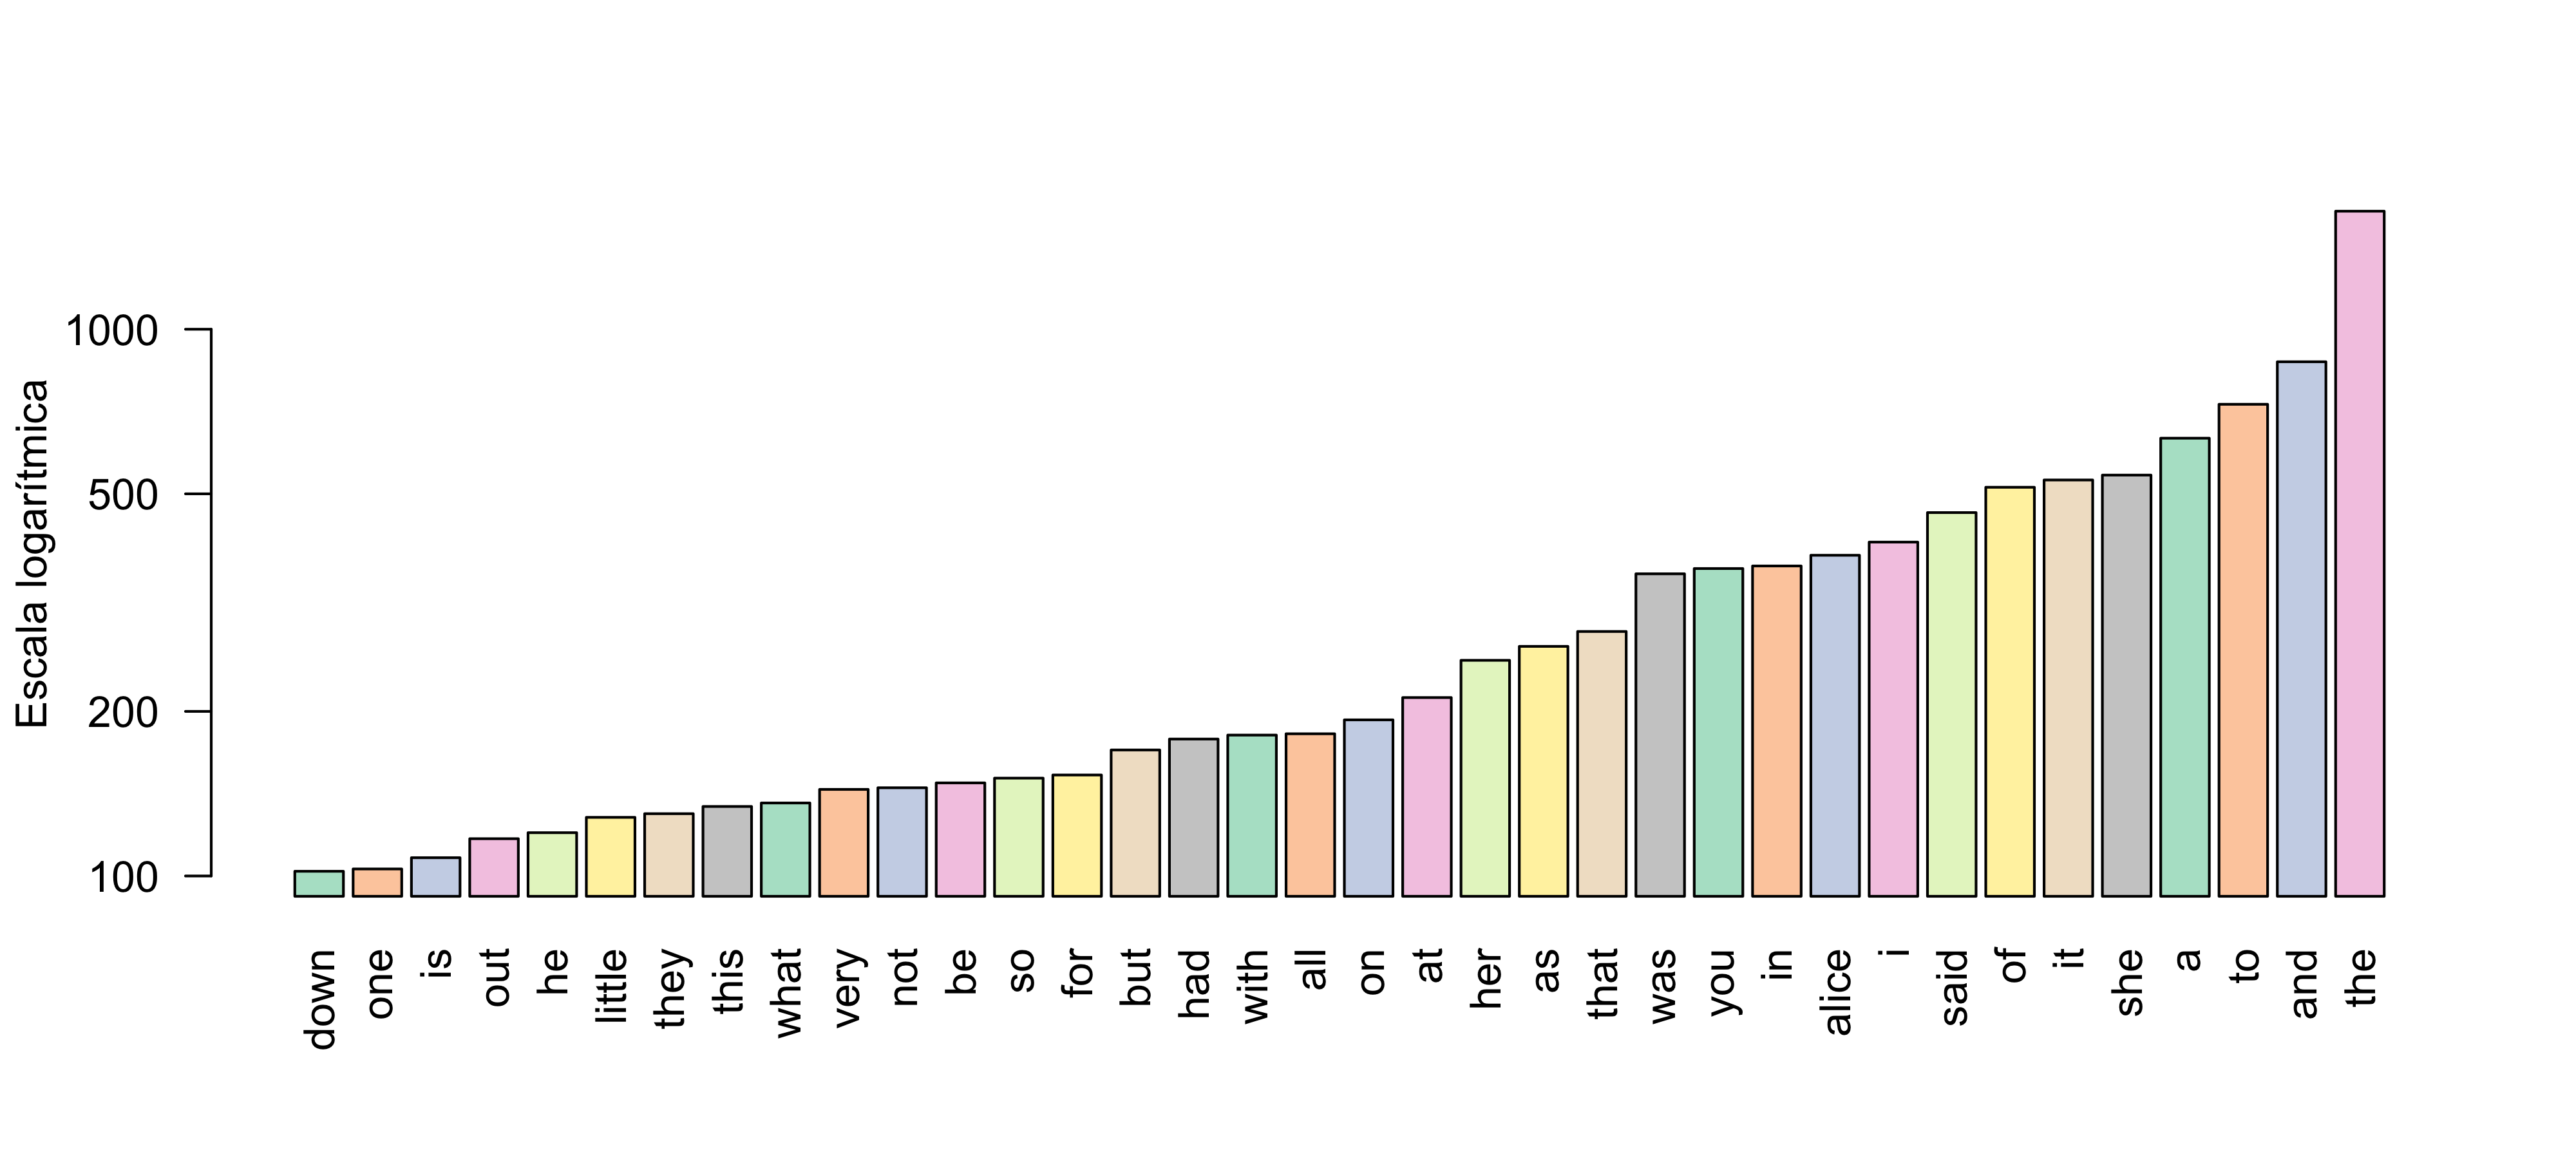
\includegraphics[scale=0.1]{Palabras.png}
\end{figure}
\begin{figure}
\centering
\caption{Palabras más frecuentes en el libro omitiendo pronombres y artículos.}
\label{Palabrasmas}
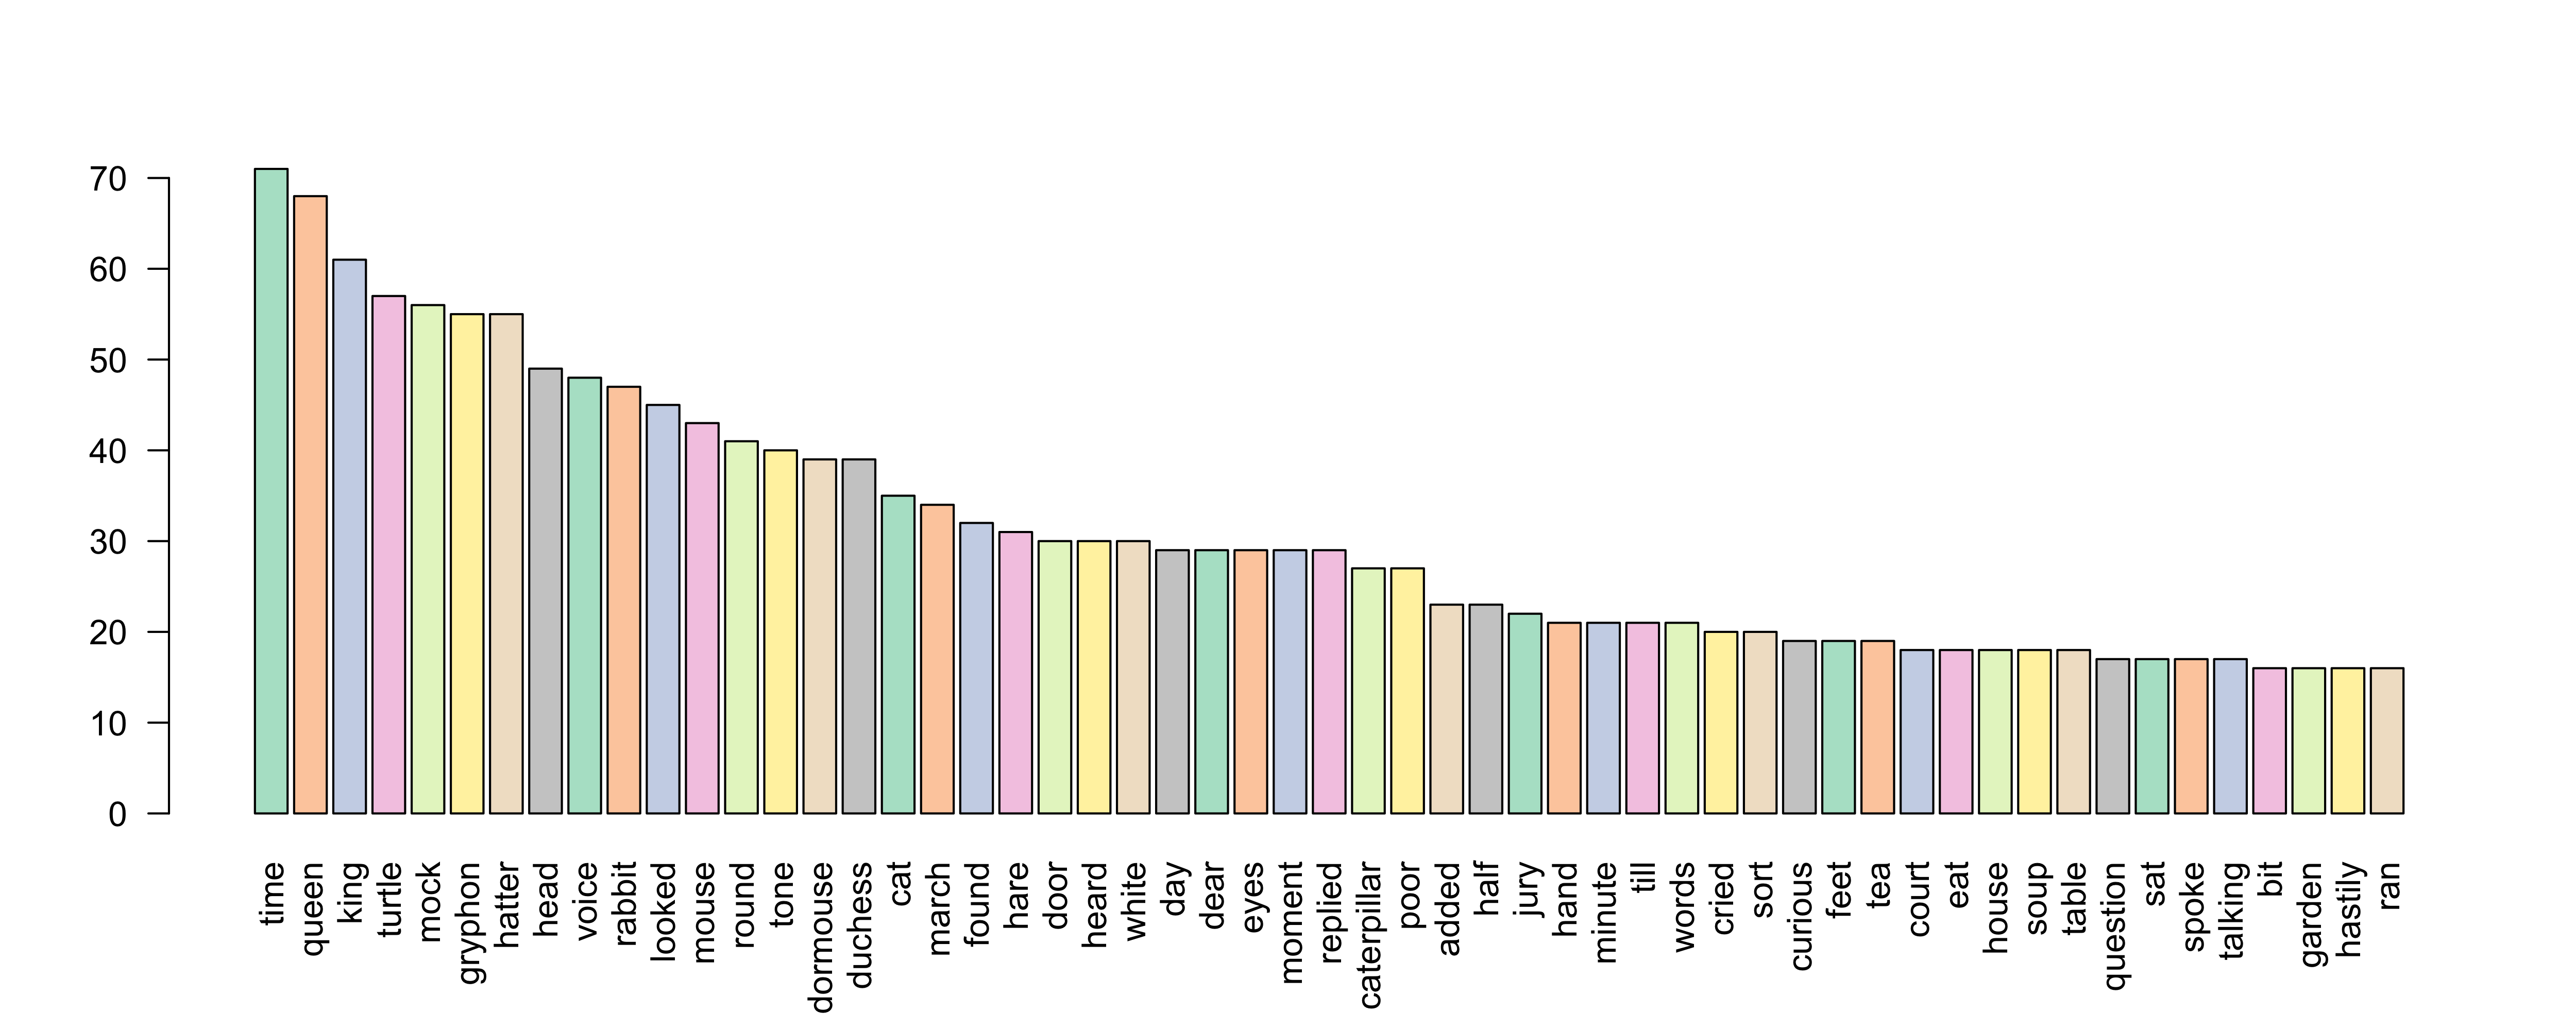
\includegraphics[scale=0.09]{Palabramss.png}
\end{figure}
\begin{figure}
\centering
\caption{Wordcloud con las palabras más frecuentes en el libro.}
\label{cloudpalabras}
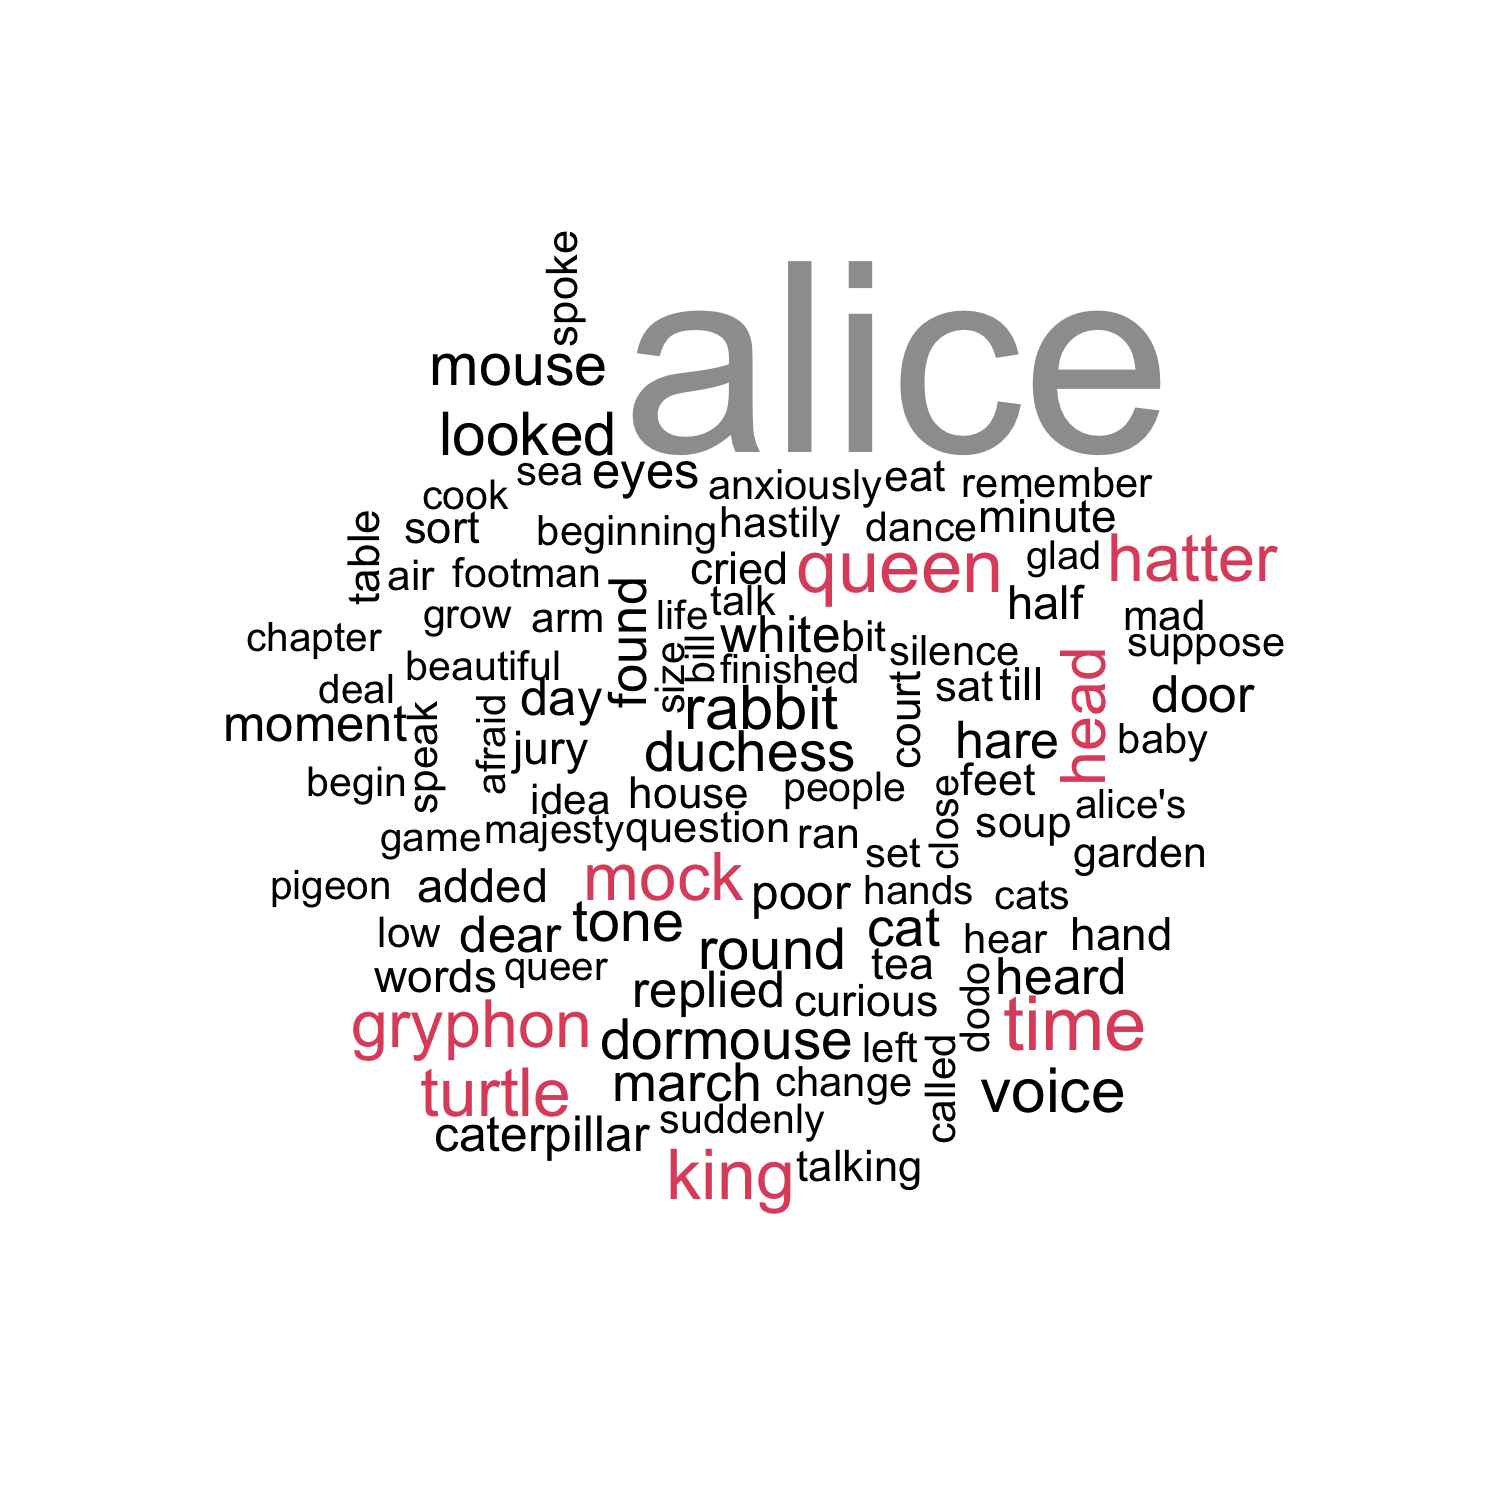
\includegraphics[scale=0.2]{cloudpalabrasmas.png}

\end{figure}
\subsection{Personajes}
El libro cuenta con una gran variedad de personajes. En este análisis consideramos solo aquellos que son más relevantes en la trama. La figura \ref{Personajes} muestra que el nombre del personaje que se menciona más durante la trama del libro es \textbf{Alice}. Los nombres de los demás personajes se mencionan de manera similar entre sí, pero con menor frecuencia que la del personaje principal.

\begin{figure}
\centering
\caption{Personajes más frecuentes en el libro.}
\label{Personajes}
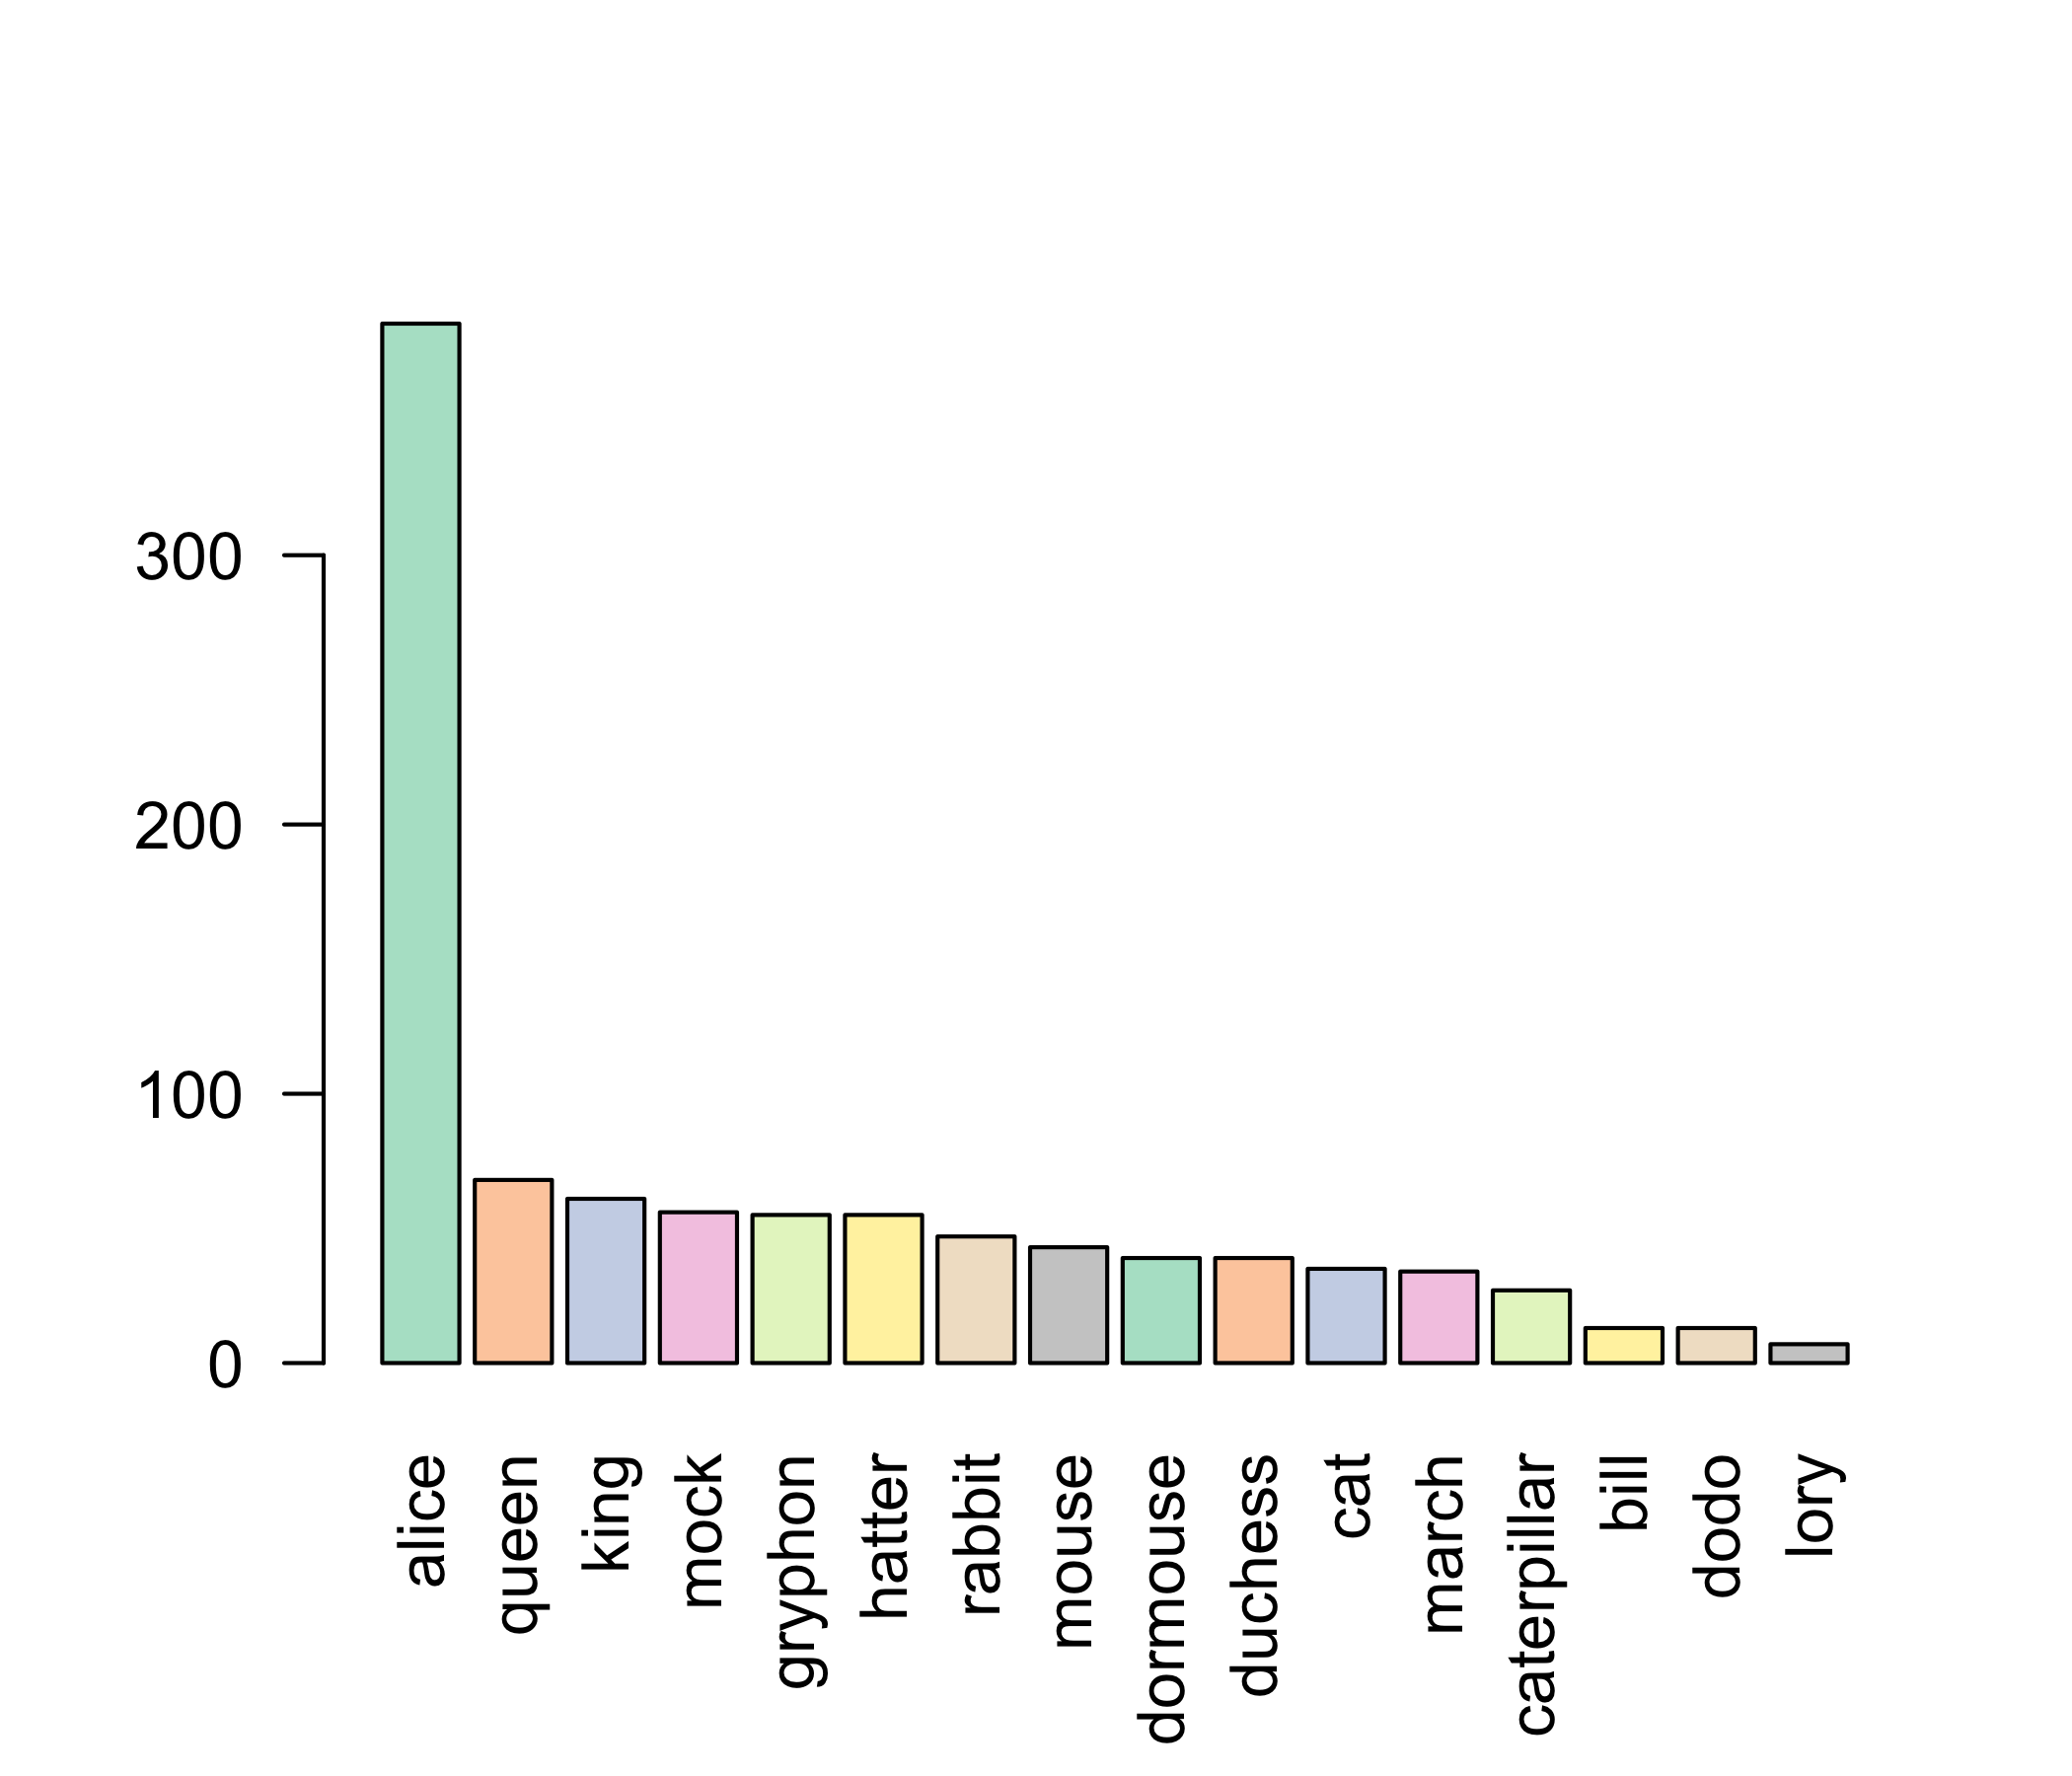
\includegraphics[scale=0.16]{Personajes.png}
\end{figure}


\subsection{Análisis de los sentimientos}
Una novela puede transmitir diversos sentimientos, dependiendo del tipo de novela que es. Para este análisis es necesario una librería que nos permite acceder a diversos diccionarios que contienen palabras asociadas a ciertos sentimientos, o clasificadas como sentimientos positivos o negativos.

En la figura \ref{positivonegativo} podemos apreciar una comparación entre los sentimientos negativos y positivos que se encuentran en el libro. Como vemos, el lado izquierdo, referente a los negativos, tiene palabras más frecuentes que el apartado derecho, es decir que se habla más de sentimientos negativos.
\begin{figure}
\centering
\caption{Comparación de sentimientos positivos y negativos.}
\label{positivonegativo}
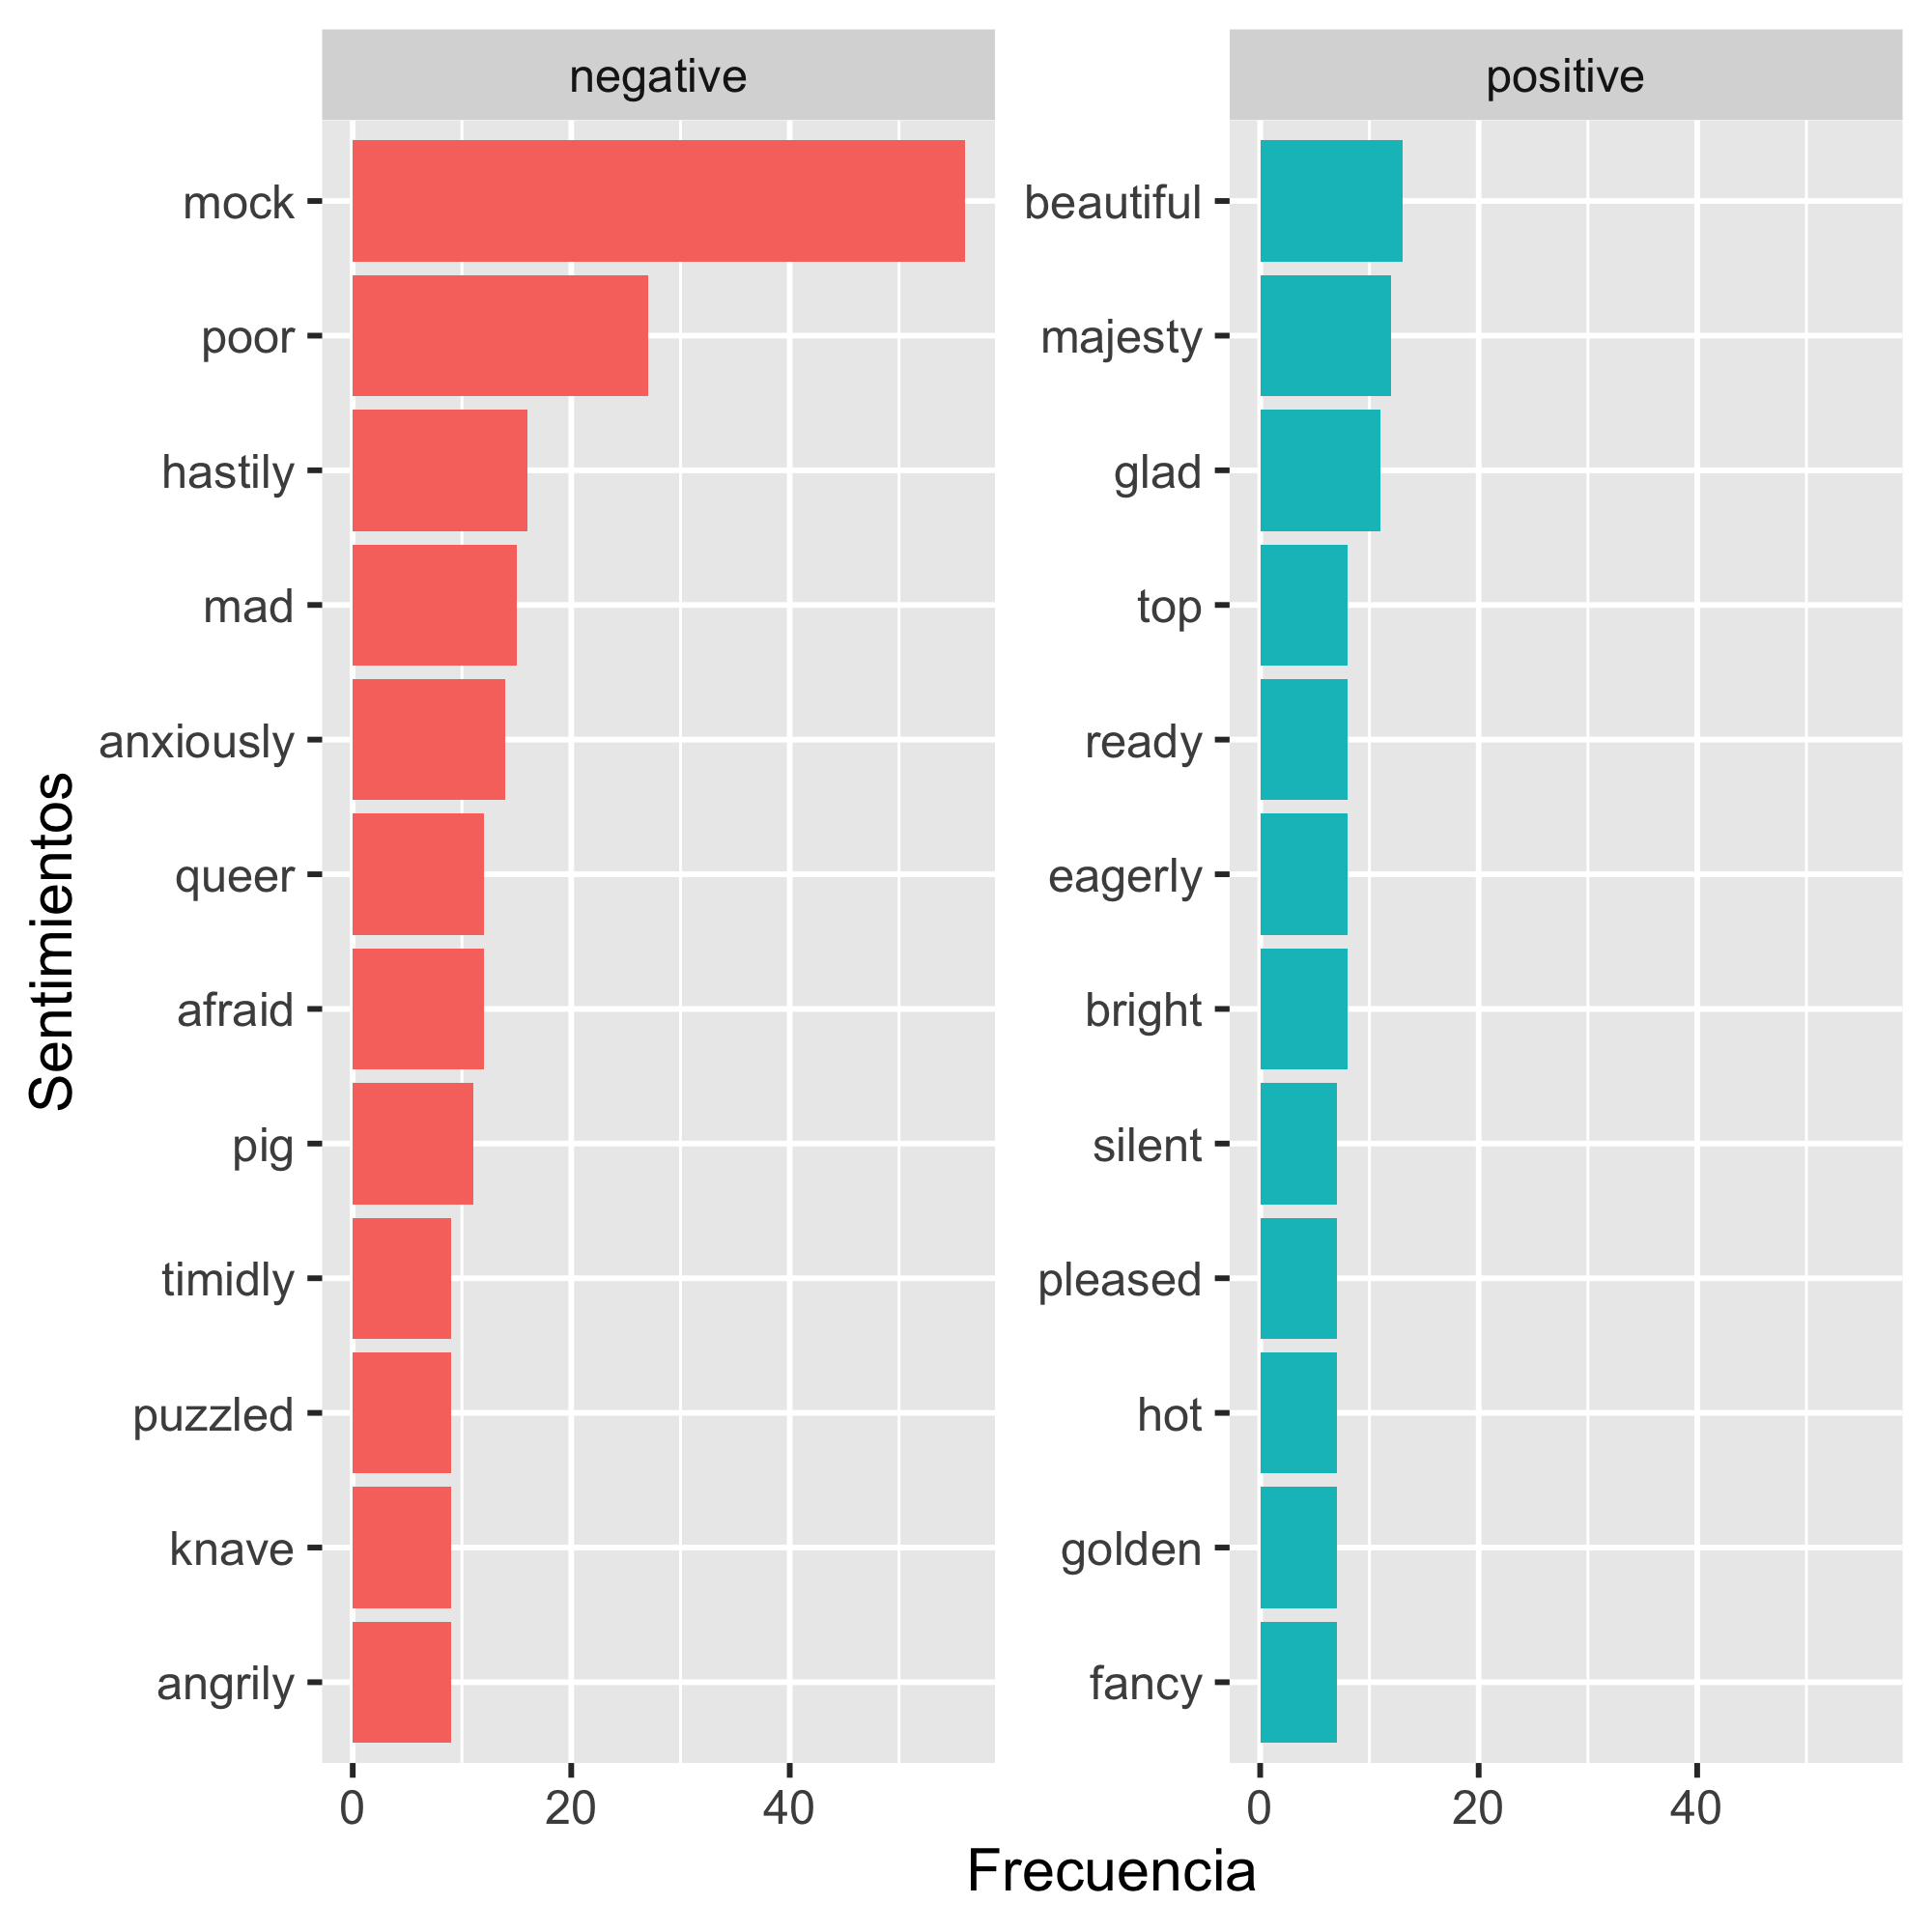
\includegraphics[scale=0.2]{positivo-negativo.png}
\end{figure}

\begin{figure}
\centering
\caption{Wordcloud comparativo entre sentimientos negativos y positivos.}
\label{negposit}
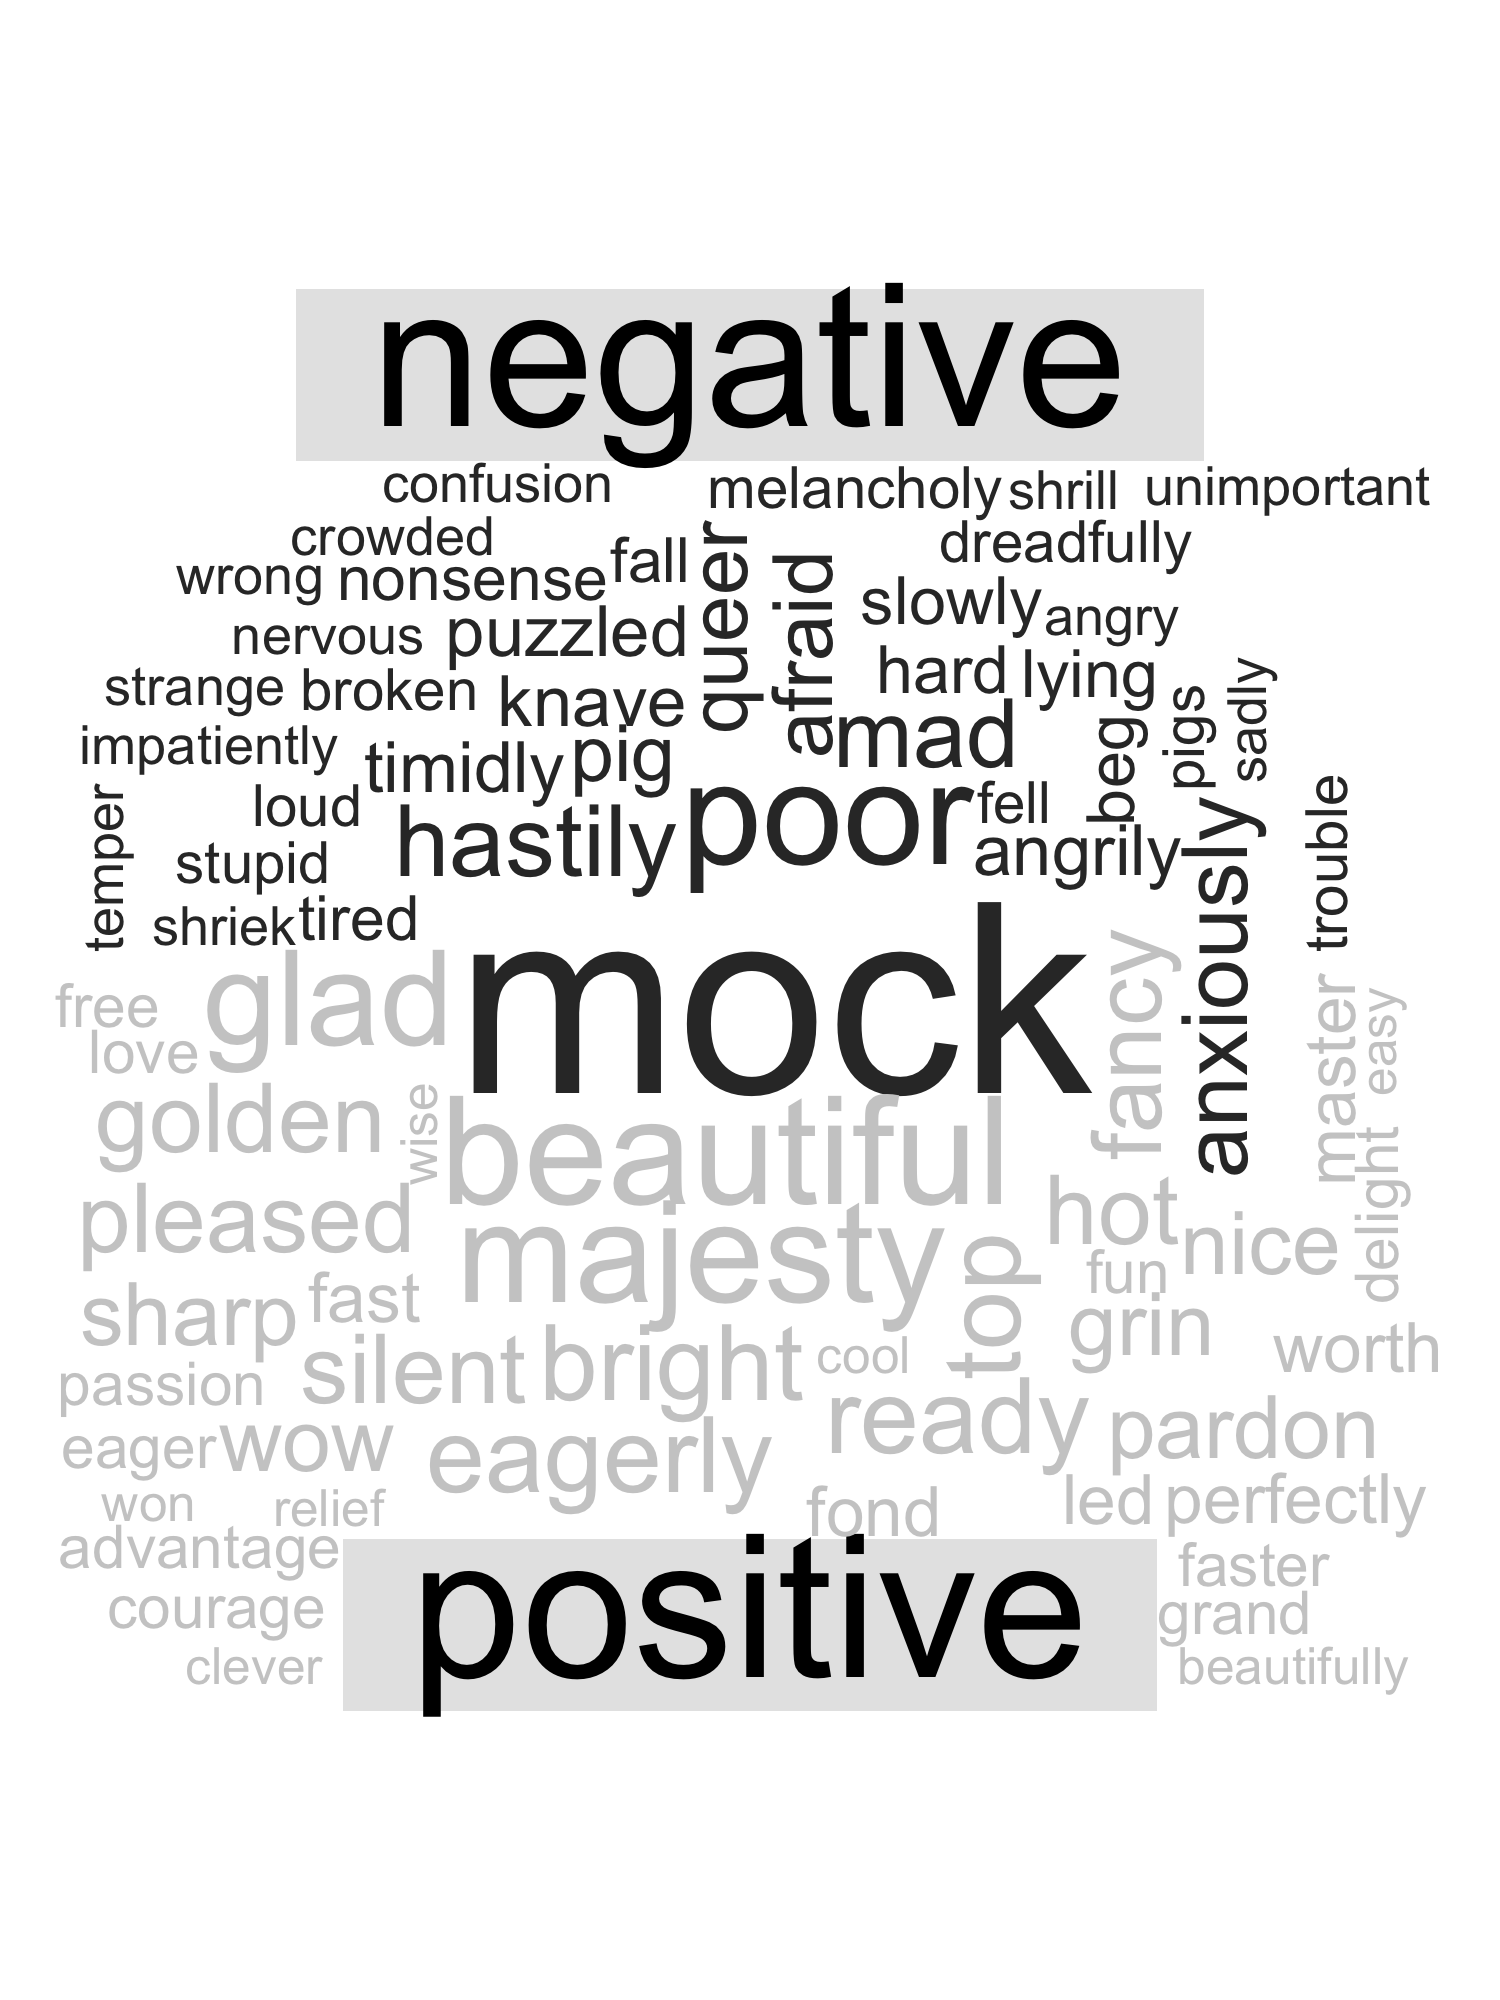
\includegraphics[scale=0.15]{cloud.png}
\end{figure}


\section{Conclusiones}
Este tipo de análisis de textos es muy útil ya que te ayuda a obtener información importante del texto que se analiza. Por ejemplo, las palabras más frecuentes en el libro (omitiendo pronombres, artículos, conectores) nos sirven para darnos una idea sobre la trama del texto.



\bibliographystyle{plain} 
\bibliography{Referencias}
\end{document}